% \section{Anexos}

% % === TEXTO ORIGINAL CORREGIDO ===
% Anexo 1: Diagrama de flujo

% % === FIGURA 2 ===
% \begin{figure}[H] % H mayúscula fuerza posición exacta
%     \centering
%     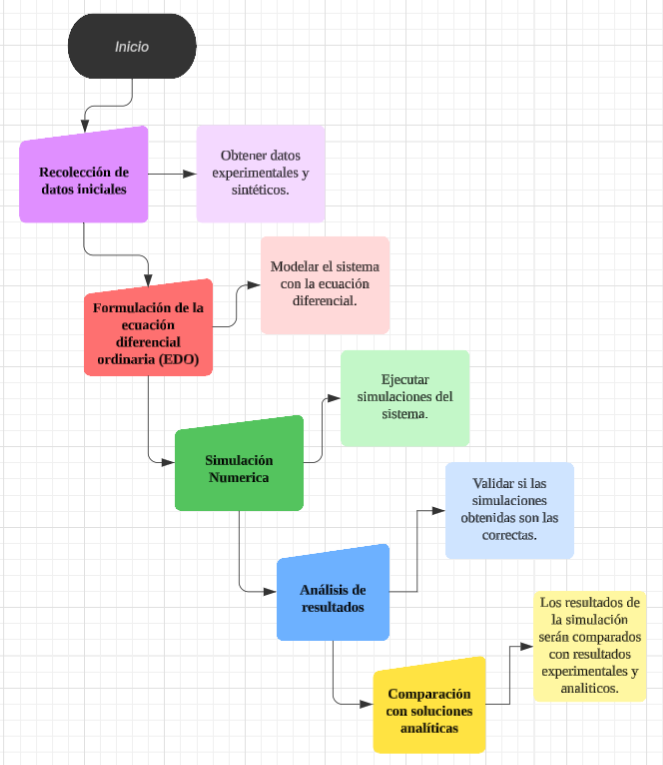
\includegraphics[width=0.8\textwidth]{5.png}
% \end{figure}
% Anexo 2: Código y gráfica de la carga en el capacitor vs. Tiempo

% % === FIGURA 3 ===
% \begin{figure}[h]
%     \centering
%     % añadir aca
% \end{figure}
\section{Anexos}
\vspace*{2cm}
Anexo 1: Diagrama de flujo
\begin{figure}[H]
	\centering
	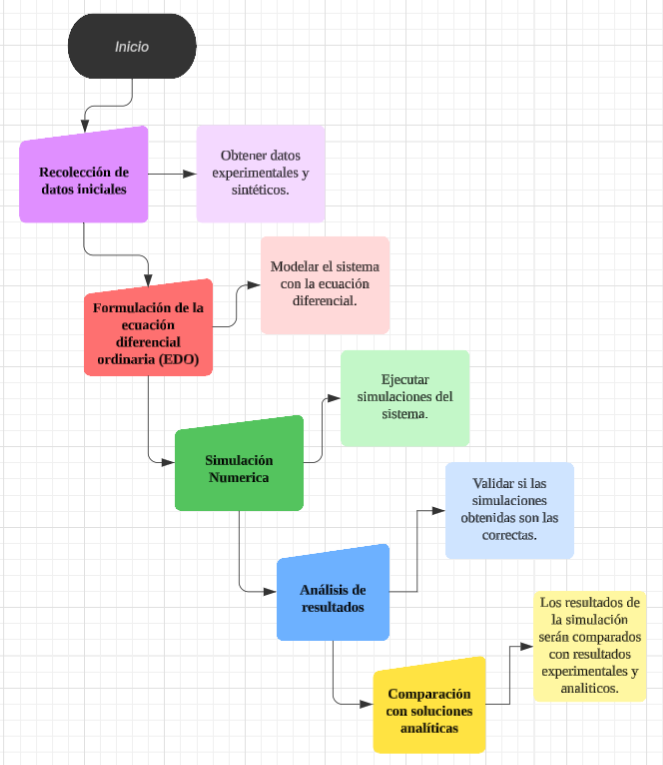
\includegraphics[width=0.8\textwidth]{5.png}
\end{figure}
\newpage
Anexo 2: Código y gráfica de la carga en el capacitor vs. Tiempo

\begin{figure}[H]
	\centering
	% Espacio para tu imagen (reemplaza "grafica_carga.png" con tu archivo)
	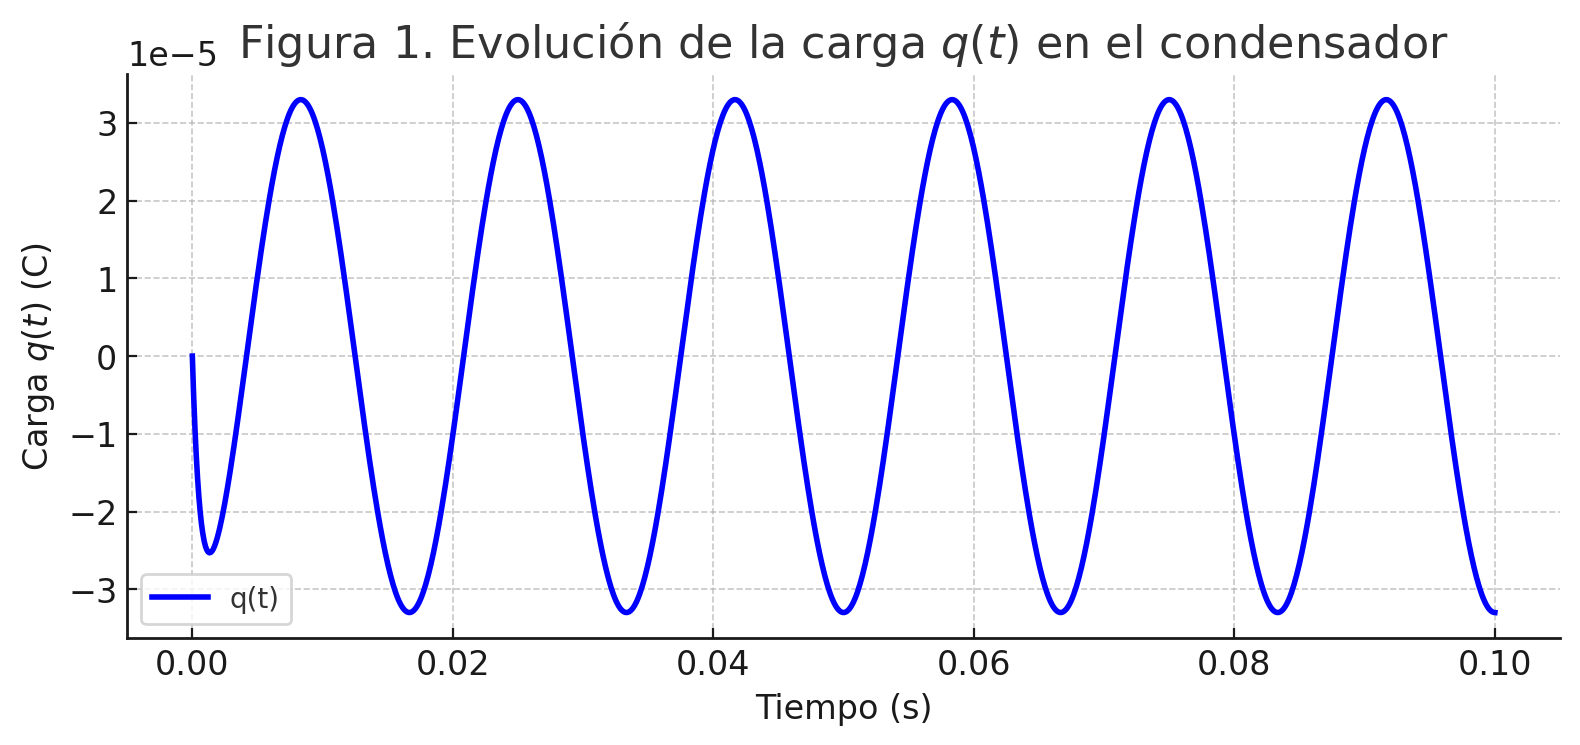
\includegraphics[width=0.8\textwidth]{7.png}
	\caption{Gráfica generada con Python}
\end{figure}

\begin{lstlisting}[language=Python, caption={Código Python para simulación de carga}, label={cod:python}, frame=single, basicstyle=\footnotesize\ttfamily]
import numpy as np
import matplotlib.pyplot as plt
R_bat = 0.2      # Resistencia interna de la batería (ohmios)
R_x = 0.1        # Resistencia del sistema (ohmios)
R_c = 0.3        # Resistencia de control o convertidor (ohmios)
C = 1000e-6      # Capacitancia (faradios)
omega = 2 * np.pi * 60  # Frecuencia angular (60 Hz)

tau = C * (R_bat + R_x + R_c)

A = 3.2982e-5
B = 5.4679e-8
C_p = -3.2982e-5

t = np.linspace(0, 0.1, 1000)
q_t = A * np.exp(-t / tau) + B * np.sin(omega * t) + C_p * np.cos(omega * t)

plt.figure(figsize=(8, 4))
plt.plot(t, q_t, label='q(t)', color='blue', linewidth=2)
plt.title('Carga en el Capacitor vs. Tiempo')
plt.xlabel('Tiempo (s)')
plt.ylabel('Carga q(t) (C)')
plt.grid(True)
plt.legend()
plt.tight_layout()
plt.show()
\end{lstlisting}

\newpage
Anexo 3: Código y gráfica del análisis espectral de la señal q(t) mediante FFT

\begin{figure}[H]
	\centering
	% Espacio para tu imagen (reemplaza "grafica_carga.png" con tu archivo)
	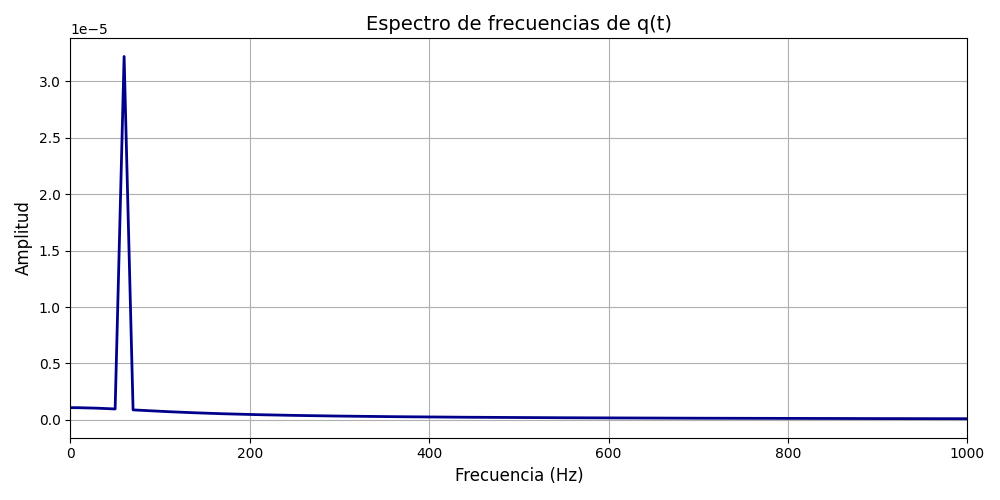
\includegraphics[width=0.8\textwidth]{8.png}
	\caption{Gráfica generada con Python}
\end{figure}

\begin{lstlisting}[language=Python, caption={Código Python del análisi espectral}, label={cod:python}, frame=single, basicstyle=\footnotesize\ttfamily]
import numpy as np
import matplotlib.pyplot as plt
from scipy.fft import fft, fftfreq

# Parámetros del sistema
tau = 1.6e-3              # Constante de tiempo (s)
omega = 2 * np.pi * 60    # Frecuencia angular (60 Hz)
f_s = 10000               # Frecuencia de muestreo (Hz)
T = 1 / f_s               # Periodo de muestreo
t = np.arange(0, 0.1, T)  # Tiempo de 0 a 0.1 s

# Coeficientes de la señal
A = 3.2982e-5
B = 5.4679e-8
C = -3.2982e-5

# Definición de la señal q(t)
q_t = A * np.exp(-t / tau) + B * np.sin(omega * t) + C * np.cos(omega * t)

# FFT (Transformada rápida de Fourier)
N = len(t)
yf = fft(q_t)
xf = fftfreq(N, T)[:N//2]                      # Frecuencias positivas
amplitud = 2.0 / N * np.abs(yf[0:N//2])        # Magnitud normalizada

# Graficar espectro de frecuencias
plt.figure(figsize=(10, 5))
plt.plot(xf, amplitud, color='darkblue', linewidth=2)
plt.title('Espectro de frecuencias de q(t)', fontsize=14)
plt.xlabel('Frecuencia (Hz)', fontsize=12)
plt.ylabel('Amplitud', fontsize=12)
plt.grid(True)
plt.xlim(0, 1000)
plt.tight_layout()
plt.show()
\end{lstlisting}


